\section{Problem Formulation}
\label{sec:problem}

\textbf{Setting.} Let $M=(\mathcal S,\mathcal A,P,R,\gamma,\rho)$ be a finite discounted MDP with $S$ states, $A$ actions and $\gamma=0.95$. A behavior policy $\beta$ generates a pilot log $D_0$ of $N_0=10SA$ transitions in episodes of at most 100 steps. An offline \emph{learner} $l$ maps a buffer to a policy. A \emph{forecaster} maps $(D_0,l)$, public metadata ($S$, $A$, $\rho$, $\gamma$) and a model fitted on earlier \emph{meta-training} cohorts to seven probabilities $p_{l,0},\ldots,p_{l,6}$. It never sees the true MDP. Fig.~\ref{fig:pipeline} separates the forecast and label paths.

\begin{figure*}[t]
\centering
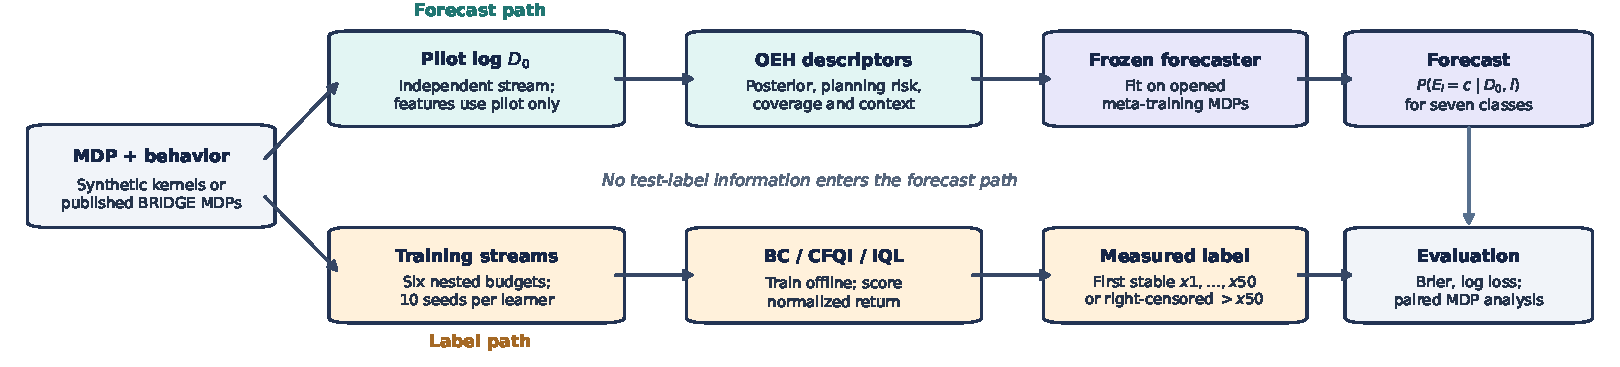
\includegraphics[width=\textwidth]{figures/oeh_pipeline.pdf}
\caption{Forecast path and label path. The pilot $D_0$ and learner identity enter the frozen forecaster; independent training streams at nested budgets and ten seeds per learner produce the measured, possibly censored requirement label. Forecasts are sealed before labels and joined only for scoring.}
\label{fig:pipeline}
\end{figure*}

\textbf{Learner-specific empirical requirement.} For a policy $\pi$ with value $J(\pi)=\rho^\top V^\pi$, the normalized return is
\begin{equation}
\mathrm{NR}(\pi)=\frac{J(\pi)-J_{\rm random}}{J^*-J_{\rm random}},
\label{eq:nr}
\end{equation}
computed exactly in the true MDP. A training seed succeeds when $\mathrm{NR}\geq\tau=0.95$. The budgets are $N_j=b_jSA$ with $b=(1,2,5,10,20,50)$, nested prefixes of each of ten independent training streams. With $\pi_{l,j,i}$ the policy of seed $i$ at budget $j$,
\begin{equation}
\begin{aligned}
C_{l,j}&=\textstyle\sum_{i=1}^{10}\mathbf 1\{\mathrm{NR}(\pi_{l,j,i})\geq\tau\},\\
E_l&=\min\bigl\{j:\min\nolimits_{m\geq j}C_{l,m}\geq 8\bigr\},
\end{aligned}
\label{eq:event}
\end{equation}
with $E_l=6$ ($>x50$) when no index qualifies. The suffix condition handles non-monotone learning curves: counts $(2,5,8,7,9,10)$ give $E_l=4$ ($x20$), not $x5$, because success at $x5$ is not sustained at $x10$. Class 6 is right censoring beyond the measured grid. The requirement is conditional on MDP, behavior, learner, threshold and protocol; it is not an intrinsic property of $M$. Because the pilot already costs $x10$, the classes $x1$--$x5$ are retrospective; Section~\ref{sec:method} defines an endpoint restricted to the budgets beyond the pilot.

\textbf{Information access.} The pilot and training streams use disjoint seed namespaces, and the true kernel is used only to generate data and to score policies. No pilot-only statistic can identify the value of an action that was never logged: two MDPs that agree on every logged action produce the same pilot distribution. Our posterior therefore encodes a convention (unobserved reward keys receive zero), not a certificate. Comparators that use the true MDP or reference data from it are labeled \emph{privileged}.
